
\documentclass[a4paper,14pt]{extreport} % формат документа

%\documentclass[utf8x, 14pt]{G7-32}
\usepackage[warn]{mathtext}
\usepackage{amsmath}
\usepackage{cmap} % поиск в ПДФ
\usepackage[T2A]{fontenc} % кодировка
\usepackage[utf8]{inputenc} % кодировка исходного текста
\usepackage[english,russian]{babel} % локализация и переносы
\usepackage[left = 2cm, right = 1cm, top = 2cm, bottom = 2 cm]{geometry} % поля
\usepackage{listings}
\usepackage{graphicx} % для вставки рисунков
\usepackage{amsmath}
\usepackage{float}
\usepackage{longtable}
\usepackage{multirow}
\usepackage{pdfpages}
\graphicspath{{pictures/}}
\DeclareGraphicsExtensions{.pdf,.png,.jpg}
\newcommand{\anonsection}[1]{\section*{#1}\addcontentsline{toc}{section}{#1}}

\begin{document}
	
\begin{titlepage}
	
	\begin{table}[H]
		\centering
		\footnotesize
		\begin{tabular}{cc}
			\multirow{8}{*}{
\includegraphics[scale=0.35]{bmstu.jpg}}
			& \\
			& \\
			& \textbf{Министерство науки и высшего образования Российской Федерации} \\
			& \textbf{Федеральное государственное бюджетное образовательное учреждение} \\
			& \textbf{высшего образования} \\
			& \textbf{<<Московский государственный технический} \\
			& \textbf{университет имени Н.Э. Баумана>>} \\
			& \textbf{(МГТУ им. Н.Э. Баумана)} \\
		\end{tabular}
	\end{table}
	
	\vspace{-1.5cm}
	
	\begin{flushleft}
		\rule[-1cm]{\textwidth}{3pt}
		\rule{\textwidth}{1pt}
	\end{flushleft}
	
	\begin{flushleft}
		\small
		ФАКУЛЬТЕТ
		\underline{<<Информатика и системы управления>>\ \ \ \ \ \ \ 
			\ \ \ \ \ \ \ \ \ \ \ \ \ \ \ \ \ \ \ \ \ \ \ \ \ \ \ \ \ \ \ 
			\ \ \ \ \ \ \ \ \ \ \ \ \ \ \ } \\
		КАФЕДРА
		\underline{<<Программное обеспечение ЭВМ и
			информационные технологии>>
			\ \ \ \ \ \ \ \ \ \ \ \ \ \ \ \ \ \ \ \ }
	\end{flushleft}
	
	\vspace{2cm}
	
	\begin{center}
		\textbf{Лабораторная работа № 6} \\
		\textbf{Дисциплина:}  Компьютерные сети.  \\
		\textbf{Тема} 
		Разбиение сети на подсети. \\ Настройка DHCP-сервера в сетевом  эмуляторе\\
		\textbf{Вариант №15} \\
	\end{center}

    \vspace{4cm}
    
	\begin{flushright}
		\begin{tabular}{rr}
			\textbf{Студент} & Неклепаева А.Н. \\
			\textbf{Группа} & ИУ7-73Б \\
			\textbf{Преподаватель} & Рогозин Н.О.   \\
		\end{tabular}
	\end{flushright}
	
	\vspace{7cm}
	
	\begin{center}
		Москва, 2020 г.
	\end{center}
	
\end{titlepage}

\textbf{Задача:} для локальной общей сети был выделен частный адрес 192.168.15.0/24

I. Разделить сеть на 5 подсетей

1) Подсети 1 и 5 должны поддерживать до 15 + 10 устройств;

2) Подсети 2 и 4 должны поддерживать до 5 устройств;

3) Подсеть 3 должна поддерживать только 2 устройства.

Использовать не более трех подсетей с возможностью размещения 15 +
10 хостов.

II. Настроить DHCP-сервера для выдачи адресов

1) Для подсети 1 настроить отдельный DHCP сервер;

2) Для подсети 2 настроить в качестве DHCP-сервера маршрутизатор 1;

3) Для подсетей 4, 5 настроить в качестве DHCP-сервера маршрутизатор 2.

\textbf{Результаты работы:}

Разбиение сети на подсети начинается с подсетей с наибольшим количеством устройств. 

192.168.15.0 – 11000000.10101000.00001111.00000000

Маски для подсетей 1 и 5:

$ 2^{5} - 2 \geq 25 $

$ 30 \geq 25 \Longrightarrow 11111111.11111111.11111111.11100000 (/27)$ или $ 224 $

Для адресации используются 5 битов.
К маске  добавляются еще биты 7-5, поэтому имеем маску /27.

\underline{Первая подсеть:}

IP-адрес подсети 192.168.15.0

Широковещательный адрес подсети 192.168.15.31

Диапазон адресов 192.168.15.1 - 192.168.15.30

\underline{Пятая подсеть:}

IP-адрес подсети 192.168.15.32

Широковещательный адрес подсети 192.168.15.63

Диапазон адресов 192.168.15.33 - 192.168.15.62

Маски для подсетей 2 и 4:

$ 2^{3} - 2 \geq 5 $

$ 6 \geq 5 \Longrightarrow 11111111.11111111.11111111.11111000 (/29)$ или $ 248 $

\underline{Вторая подсеть:}

IP-адрес подсети 192.168.15.64

Широковещательный адрес подсети 192.168.15.71

Диапазон адресов 192.168.15.65 - 192.168.15.70

\underline{Четвертая подсеть:}

IP-адрес подсети 192.168.15.72

Широковещательный адрес подсети 192.168.15.79

Диапазон адресов 192.168.15.73 - 192.168.15.78

Маска для подсети 3:

$ 2^{2} - 2 \geq 2 $

$ 2 \geq 2 \Longrightarrow 11111111.11111111.11111111.11111100 (/30)$ или $ 252 $

\underline{Третья подсеть:}
IP-адрес подсети 192.168.15.80

Широковещательный адрес подсети 192.168.15.83

Диапазон адресов 192.168.15.81 - 192.168.15.82

\underline{Настройка dhcp на роутере на примере сети 2:}

ip dhcp pool serverPool2 - создание пула адресов

network 192.168.15.63 255.255.255.248 - указание на диапазон адресов выдачи с данной маской

default-router 192.168.15.70 - адрес роутера в пределах сети

Шлюз по умолчанию - 192.168.15.70

IPv4-адрес у сервера - 192.168.15.70

Маска подсети - 255.255.255.248

IP-адреса конечным узлам в рамках подсети выдаются
автоматически из диапазона сетей подсети 2.
Аналогичные действия были проведены для подсетей 4 и 5. В результате маршрутизатор 2 был настроен в качестве DHCP-сервера
для подсетей 4 и 5.

Демонстрация связи между компьютерами в подсети 1:

\begin{figure}[H]
	\centering
	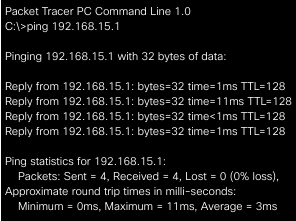
\includegraphics[width=0.7\linewidth]{1}
	\caption{}
	\label{fig:1}
\end{figure}

Демонстрация недоступности для компьютера из подсети 1 компьютера из подсети 5:
\begin{figure}[H]
	\centering
	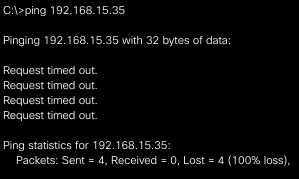
\includegraphics[width=0.7\linewidth]{2}
	\caption{}
	\label{fig:2}
\end{figure}

\end{document}
	